\documentclass[lualatex,book,paper=a4paper,jafontsize=11.5pt,jafontscale=1.05]{jlreq}

%フォント:
\usepackage{luatexja-fontspec}
\usepackage{hack-fonts}

%表紙用:
\usepackage{hack-cover}

% 画像
\usepackage{graphicx}

% 表（hyperref より先に読み込む）
\usepackage{tabularray}
\UseTblrLibrary{booktabs}
\usepackage[margin=25mm]{geometry}

% 状態遷移
\usepackage{tikz}
\usetikzlibrary{automata, positioning, arrows.meta, shapes.geometric}

% ファイル構造
\usepackage{dirtree}

% リンク（tabularray の後に読み込む）
\usepackage[hidelinks]{hyperref}

\title{ハッカソン}
\subtitle{～計画書と設計書～}
\team{チーム40}
\author{
	24G1021 : 宇井 祐真\\
        24G1026 : 梅野 大誠\\
	24G1136 : 山口 侑希 \\
        25G1020 : 薄井 悠希\\
        25G1041 : 菊池 侑人\\
        25G1059 : 佐藤 涼菜  
        }
\date{\today}
\version{x.x}

%%%%%%%%%%%%%%%%%%%%%%%%%%%%%%%%%%%%%%%%%%%%%%%%
\begin{document}
\maketitle

\setcounter{tocdepth}{2}
\tableofcontents \thispagestyle{empty}

%%%%%%%%%%%%%%%%%%%%%%%%
%%%%%%%%%%%%%%%%%%%%%%%%
%%%%%%%%%%%%%%%%%%%%%%%%
\chapter{プロジェクトの計画書} \label{chap:project-plan}\setcounter{page}{1}


%%%%%%%%%%%%%%%%%%%%%%%%
\section{プロジェクトの概要}
%%%%%%%%%%%%%%%%%%%%%%%%
\subsection{プロジェクトの題目}

%%%%%%%%%%%%%%%%%%%%%%%%
\subsection{プロジェクトの目的}
プロジェクトの目的と最終的なゴール，解決すべき課題を記述する．

%%%%%%%%%%%%%%%%%%%%%%%%
\subsection{既存の技術とプロジェクトの独自性}

%%%%%%%%%%%%%%%%%%%%%%%%
%%%%%%%%%%%%%%%%%%%%%%%%
\section{スコープ・マネジメント}
%%%%%%%%%%%%%%%%%%%%%%%%
\subsection{成果物}

%%%%%%%%%%%%%%%%%%%%%%%%
\subsection{プロジェクトの対象範囲と非対象範囲}

%%%%%%%%%%%%%%%%%%%%%%%%
\subsection{機能分解構造FBS}

%%%%%%%%%%%%%%%%%%%%%%%%
\subsection{製品分解構造PBS}

%%%%%%%%%%%%%%%%%%%%%%%%
\subsection{FBSとPBSの対応関係}


%%%%%%%%%%%%%%%%%%%%%%%%
%%%%%%%%%%%%%%%%%%%%%%%%
\section{作業計画}
%%%%%%%%%%%%%%%%%%%%%%%%
\subsection{作業分解構造WBSと管理番号}

%%%%%%%%%%%%%%%%%%%%%%%%
\subsection{アローダイアグラムとクリティカルパス}

%%%%%%%%%%%%%%%%%%%%%%%%
\subsection{役割分担}

%%%%%%%%%%%%%%%%%%%%%%%%
\subsection{ガントチャート}


%%%%%%%%%%%%%%%%%%%%%%%%
%%%%%%%%%%%%%%%%%%%%%%%%
\section{検証と妥当性確認: V\&V計画}
%%%%%%%%%%%%%%%%%%%%%%%%
\subsection{プロジェクトの成果物に対する有効指標MOE}

%%%%%%%%%%%%%%%%%%%%%%%%
\subsection{有効指標MOEに対応する性能指標MOP}

%%%%%%%%%%%%%%%%%%%%%%%%
\subsection{システムテストで評価する性能指標MOP}

%%%%%%%%%%%%%%%%%%%%%%%%
\subsection{結合テストで評価する性能指標MOP}

%%%%%%%%%%%%%%%%%%%%%%%%
\subsection{単体テストで評価する性能指標MOP}

%%%%%%%%%%%%%%%%%%%%%%%%
\subsection{プロジェクト中に監視する技術性能指標TPM}

%%%%%%%%%%%%%%%%%%%%%%%%
\subsection{プロジェクト中に監視する指標TPM}


%%%%%%%%%%%%%%%%%%%%%%%%
%%%%%%%%%%%%%%%%%%%%%%%%
\section{資源・調達管理}


%%%%%%%%%%%%%%%%%%%%%%%%
%%%%%%%%%%%%%%%%%%%%%%%%
\section{リスク管理}


%%%%%%%%%%%%%%%%%%%%%%%%
%%%%%%%%%%%%%%%%%%%%%%%%
%%%%%%%%%%%%%%%%%%%%%%%%
\chapter{システムの基本設計}

指揮デバイスについて説明を行う．


%%%%%%%%%%%%%%%%%%%%%%%%
\section{機能一覧}
% 機能分解構造FBSの要素の説明
・無線通信によるデータ転送:指揮デバイスを上下に振ることによってドラム(Arduino)にBPM情報を送信．\\
・楽曲の音量制御：つまみを動かすことで楽曲の音量を調整．
%%%%%%%%%%%%%%%%%%%%%%%%
\section{システム構成図}
% ハードウェア，ソフトウェアなどの構成図を記載する．
指揮デバイスによるBPM情報の送信方法を図\ref{fig:siki-device}に，
指揮デバイスによる音量制御方法を図\ref{fig:siki-device_big}に示す．

\begin{figure}[htbp] % h:ここ, t:上, b:下, p:独立ページ
        \centering % 中央揃え
        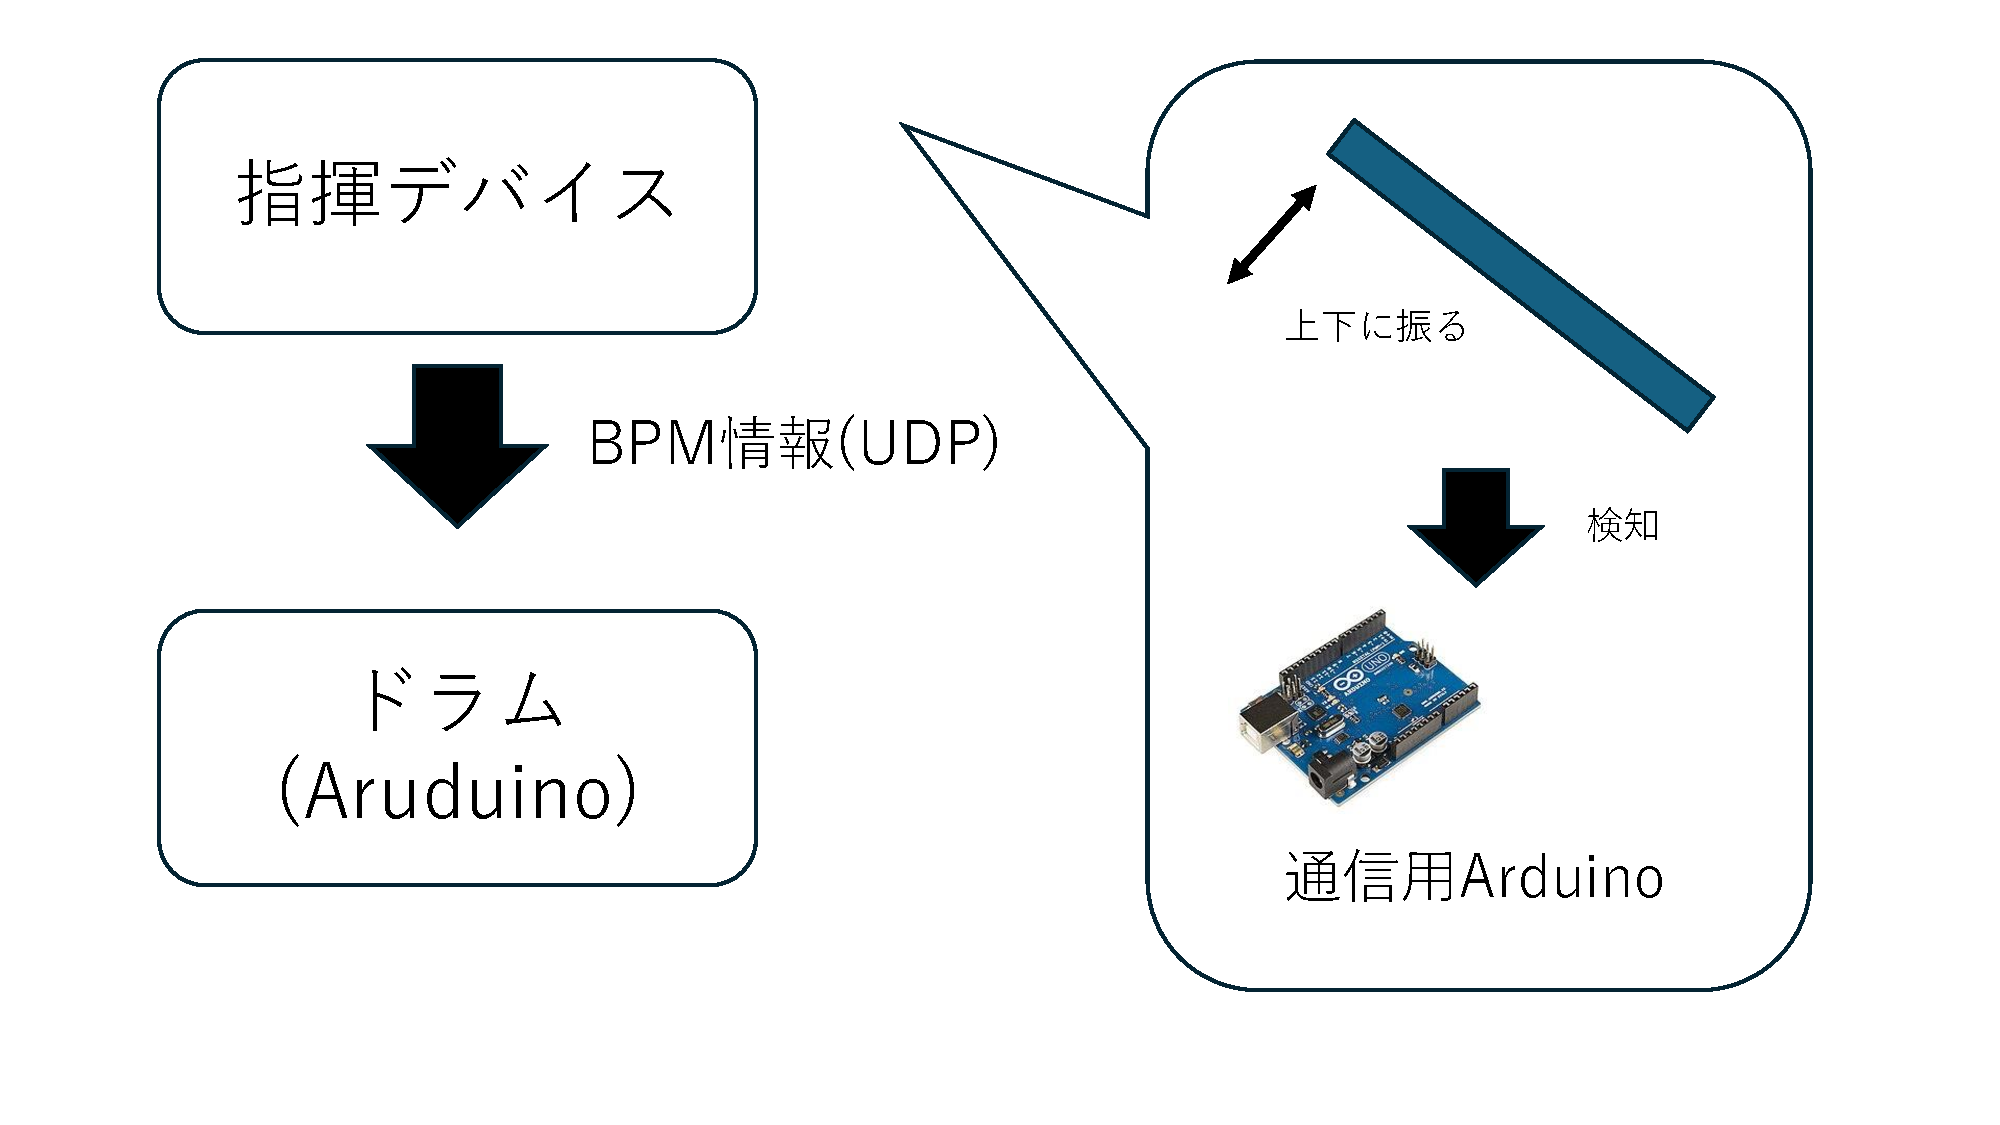
\includegraphics[width=0.8\columnwidth]{指揮デバイス_通信.pdf} % 横幅を列幅の80%に指定
        \caption{指揮デバイスとドラムArduinoの接続} % 図の説明
        \label{fig:siki-device} % 本文中で参照するためのラベル
\end{figure}

\begin{figure}[htbp] % h:ここ, t:上, b:下, p:独立ページ
        \centering % 中央揃え
        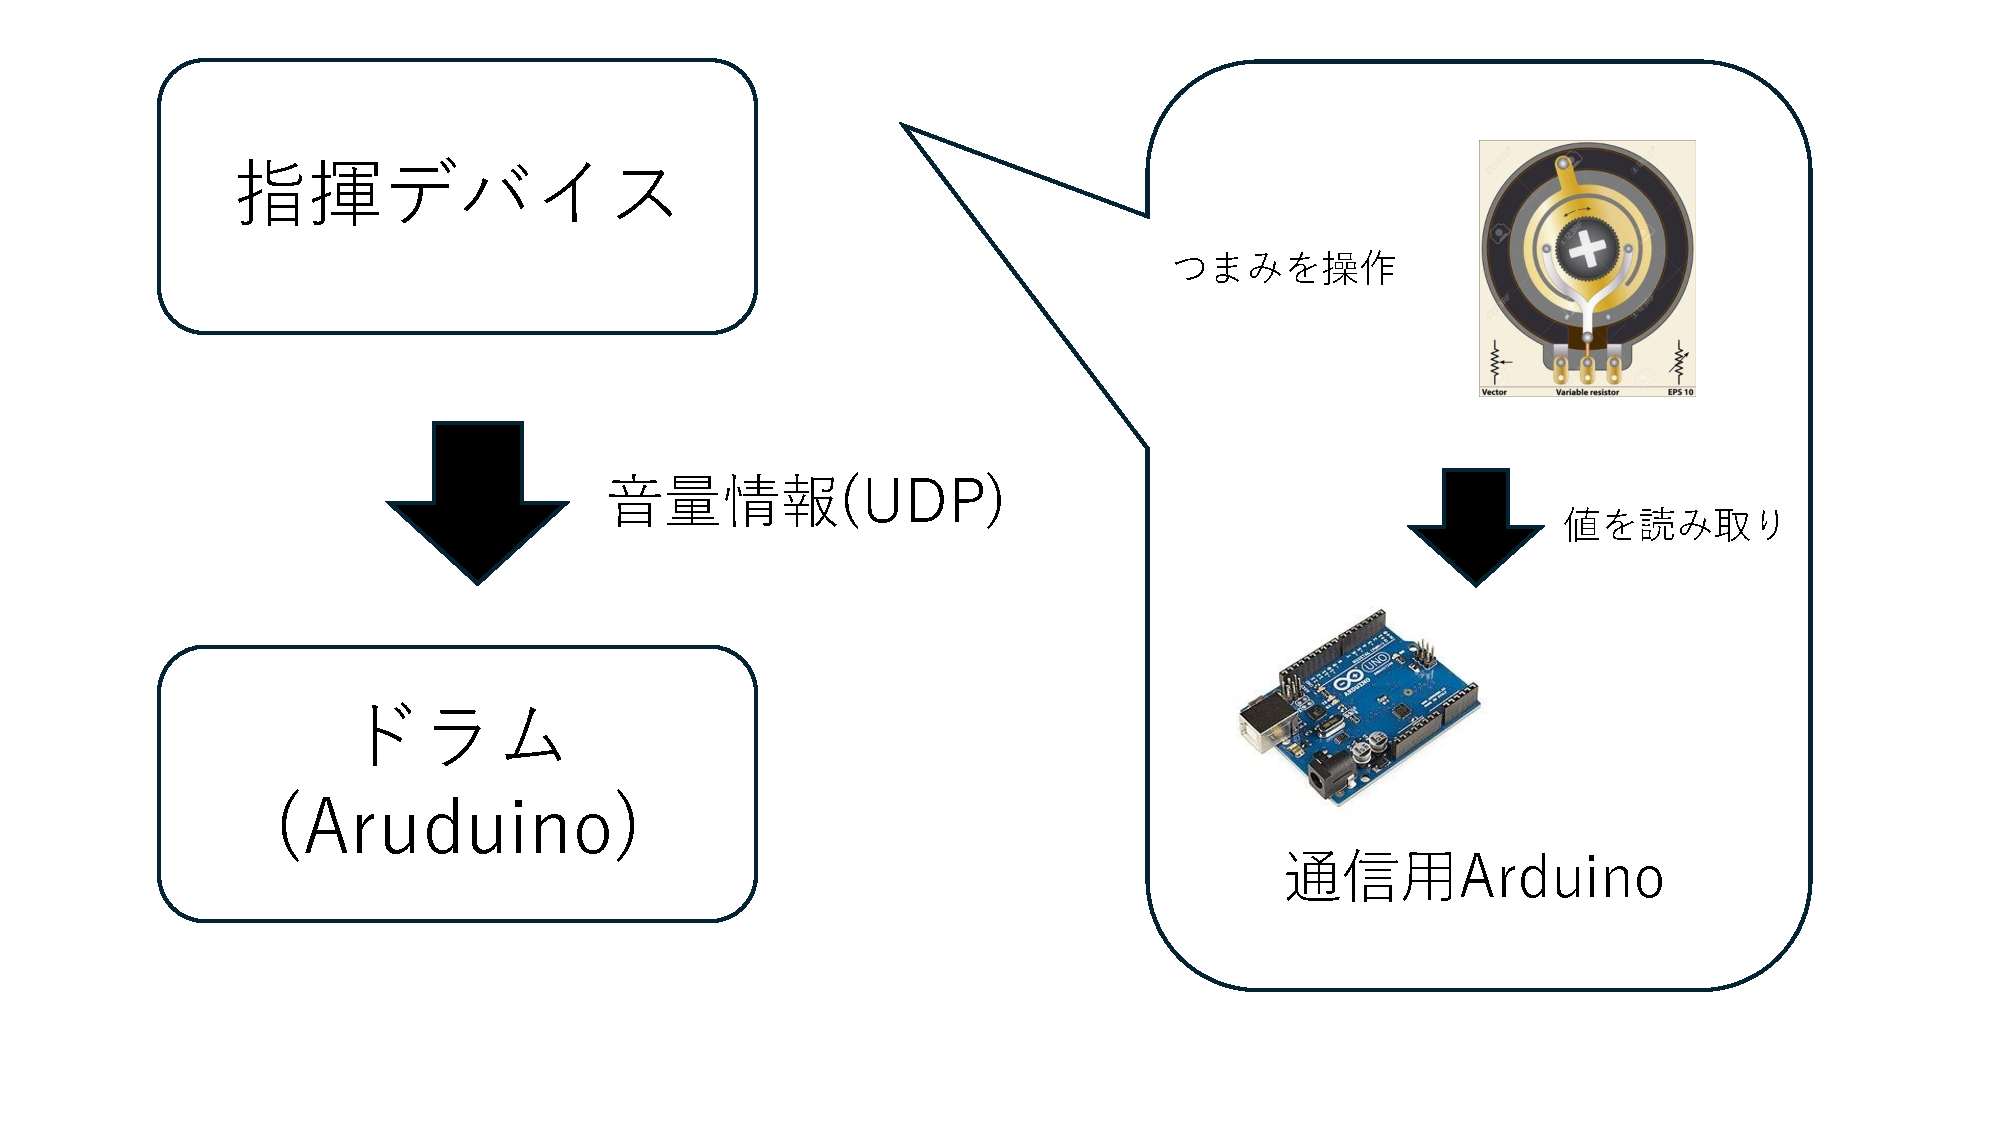
\includegraphics[width=0.8\columnwidth]{指揮デバイス_音量.pdf} % 横幅を列幅の80%に指定
        \caption{指揮デバイスによる音量調整} % 図の説明
        \label{fig:siki-device_big} % 本文中で参照するためのラベル
\end{figure}


%%%%%%%%%%%%%%%%%%%%%%%%
\section{操作インターフェース設計}
% 画面やスイッチなどのインターフェースの設計図を記載する
指揮デバイスの概要図を図\ref{fig:siki-device_zu}に示す．
また，指揮デバイスの操作に関する定義を表\ref{tab:operation_definition}に示す．

\begin{figure}[htbp] % h:ここ, t:上, b:下, p:独立ページ
        \centering % 中央揃え
        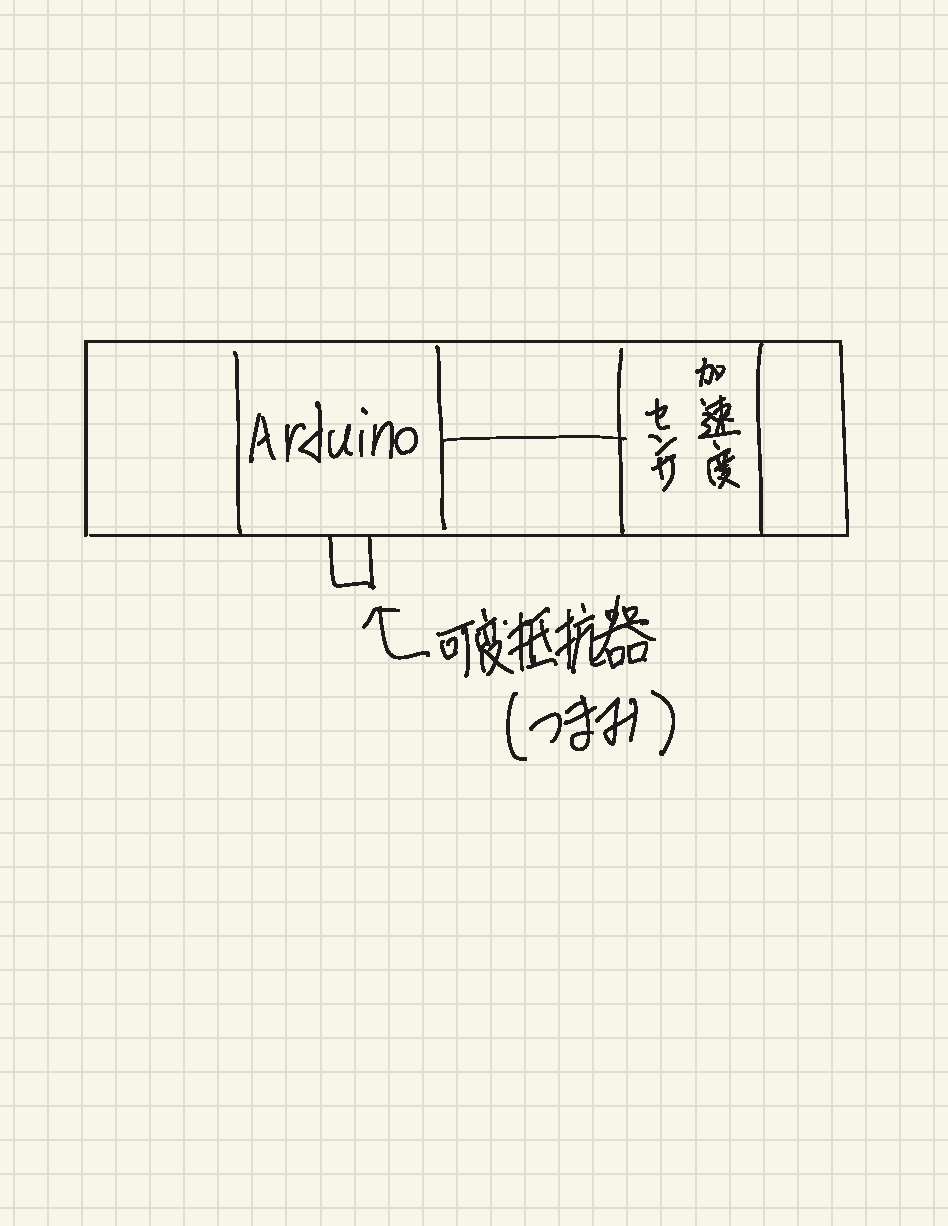
\includegraphics[width=0.8\columnwidth]{操作インターフェース.pdf} % 横幅を列幅の80%に指定
        \caption{指揮デバイスの概要図} % 図の説明
        \label{fig:siki-device_zu} % 本文中で参照するためのラベル
\end{figure}





\begin{table}[htbp]
        \caption{指揮デバイス 操作定義一覧}
        \label{tab:operation_definition}
        \centering
        \begin{tblr}{
          width = \linewidth, % テーブル幅をページ幅に合わせる
          colspec = {Q[c,m,2.5cm] Q[l,m,5cm] Q[l,m,5.5cm]}, % 列幅を調整
          hlines = {1pt, solid}, % 線の太さとスタイルを指定
          vlines = {1pt, solid}, % 線の太さとスタイルを指定
          row{1} = {font=\bfseries, c}, % ヘッダーを太字・中央揃え
        }
          操作対象 & ユーザーのアクション & システムの挙動 \\
          加速度センサ & デバイスを上下に振る & 動きを検知し，設定された閾値を超えた瞬間に楽曲のBPM情報をドラム側へ送信． \\
          可変抵抗器\par（つまみ） & つまみを左右に回して絞りを調整する & アナログ値を読み取り，BPM送信とは独立して音量情報をリアルタイムに送信． \\
        \end{tblr}
\end{table}


%%%%%%%%%%%%%%%%%%%%%%%%
\section{状態遷移図}
指揮デバイスの内部で処理される状態遷移について図\ref{fig:siki-device_senni}に示す．

\begin{figure}[htbp] % h:ここ, t:上, b:下, p:独立ページ
        \centering % 中央揃え
        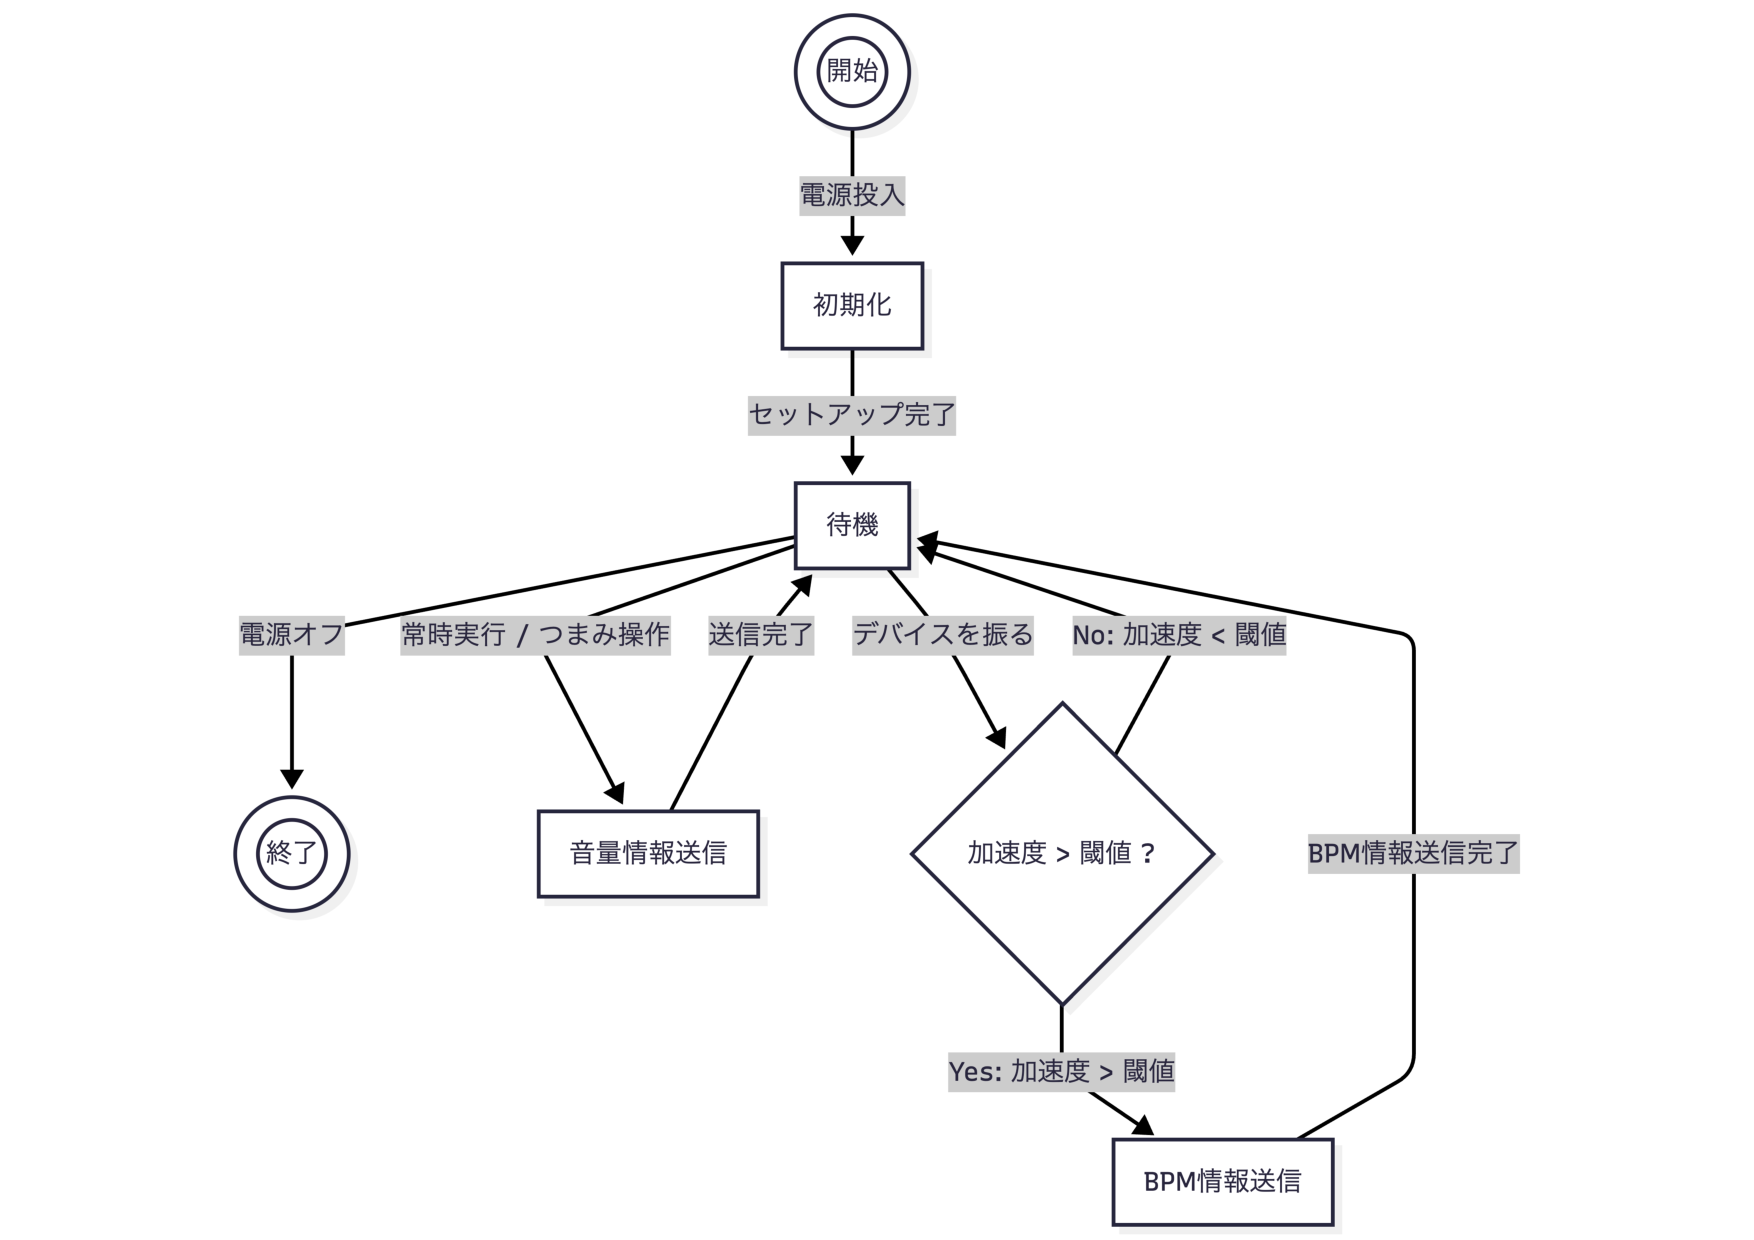
\includegraphics[width=0.8\columnwidth]{指揮デバイス_遷移.pdf} % 横幅を列幅の80%に指定
        \caption{指揮デバイス内部の状態遷移図} % 図の説明
        \label{fig:siki-device_senni} % 本文中で参照するためのラベル
\end{figure}



%%%%%%%%%%%%%%%%%%%%%%%%
%%%%%%%%%%%%%%%%%%%%%%%%
%%%%%%%%%%%%%%%%%%%%%%%%
\chapter{システムの詳細設計}

楽曲表現の詳細設計について説明を行う．

% 設計書は作成する成果物によって変化します．
% 適宜修正して利用してください．


%%%%%%%%%%%%%%%%%%%%%%%%
\section{部品一覧}
% 製品分解構造PBSの要素の説明
楽曲表現を行うにあたり必要となる部品一覧を示す．

       




%%%%%%%%%%%%%%%%%%%%%%%%
%%%%%%%%%%%%%%%%%%%%%%%%
\section{ハードウェア設計}
楽曲表現を行う箇所の回路図を図\ref{fig:hyougen}に示す．

\begin{figure}[htbp] % h:ここ, t:上, b:下, p:独立ページ
        \centering % 中央揃え
        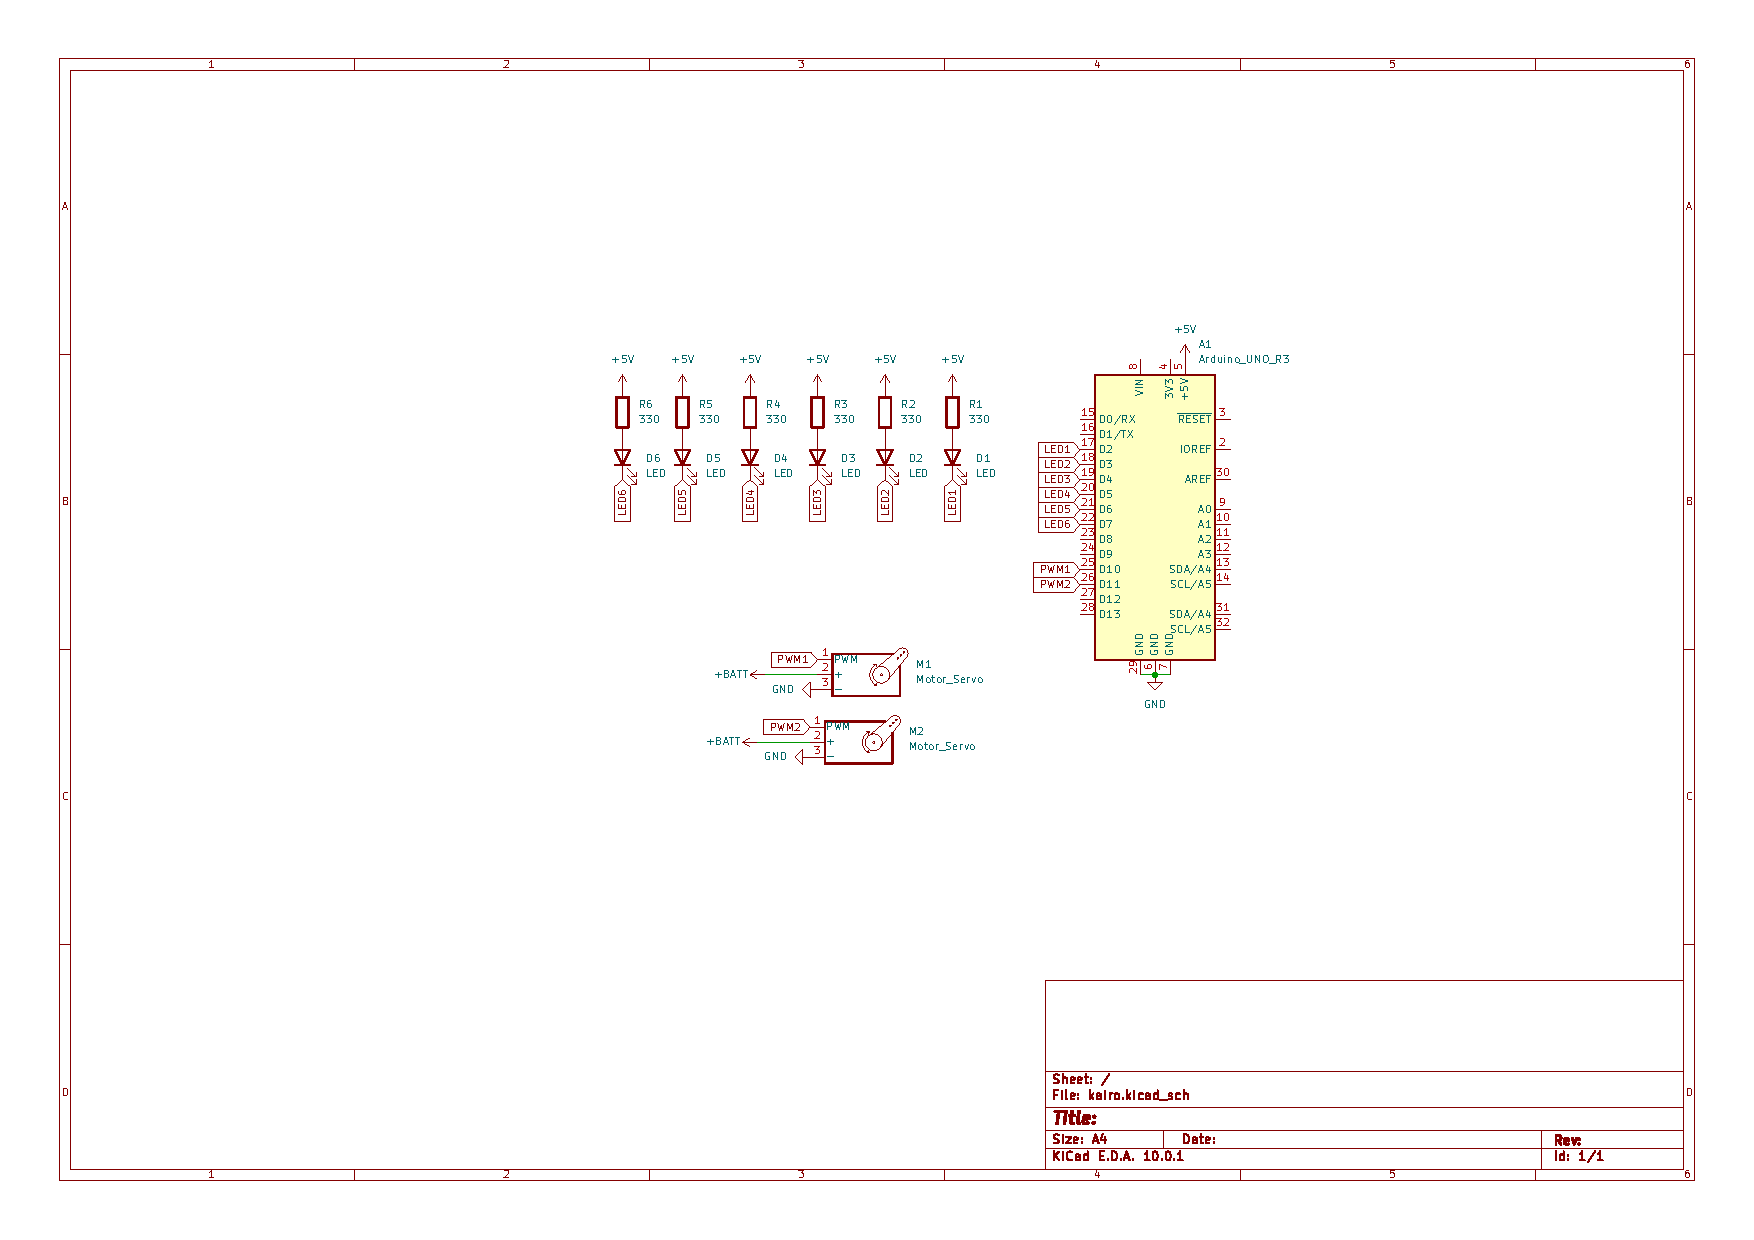
\includegraphics[width=0.8\columnwidth]{回路図.pdf} % 横幅を列幅の80%に指定
        \caption{指揮デバイス内部の状態遷移図} % 図の説明
        \label{fig:hyougen} % 本文中で参照するためのラベル
\end{figure}




%%%%%%%%%%%%%%%%%%%%%%%%
%%%%%%%%%%%%%%%%%%%%%%%%
\section{ソフトウェア設計}

%%%%%%%%%%%%%%%%%%%%%%%%
\subsection{ファイル構成}

\begin{center}
        \renewcommand{\dtstyle}{\ttfamily}
        \dirtree{%
        .1 Arduino\_orchestra/.
        .2 Arduino\_orchestra.ino \DTcomment{メインスケッチ}.
        .2 src/.
        .3 Common.h \DTcomment{共通定数・ピン定義}.
        .3 BpmUnit/ \DTcomment{BPM受信・計算}.
        .4 BpmManager.h.
        .4 BpmManager.cpp.
        .3 LedUnit/ \DTcomment{LED点灯処理}.
        .4 LedController.h.
        .4 LedController.cpp.
        .3 ServoUnit/ \DTcomment{サーボ制御}.
        .4 ServoDriver.h.
        .4 ServoDriver.cpp.
        .3 MatrixUnit/ \DTcomment{LEDマトリクス表示}.
        .4 MatrixVisualizer.h.
        .4 MatrixVisualizer.cpp.
        }
\end{center}

%%%%%%%%%%%%%%%%%%%%%%%%
\subsection{オブジェクト設計（クラス図）}

システムの各モジュールをクラスとして定義し，その構成と関係性を表\ref{tab:class_design_table}に示す．

\begin{table}[htbp]
    \caption{オブジェクト設計（クラス定義一覧）}
    \label{tab:class_design_table}
    \centering
    \begin{tblr}{
        width = \linewidth,
        colspec = {Q[l,m,3.5cm] Q[l,m,3.5cm] Q[l,m,8.5cm]},
        hlines = {1pt, solid, black},
        vlines = {1pt, solid, black},
        row{1} = {font=\bfseries, c},
    }
        クラス名 & 種別 & 内容 \\
        \texttt{BpmManager} & 属性 &
          \texttt{bpm : int} \par
          \texttt{lastBeatTime : unsigned long} \\
        & 操作 &
          \texttt{+ setBpm(bpm : int) : void} \par
          \texttt{+ isBeatTick() : bool} \par
          \texttt{+ getProgress() : float} \\
        \texttt{LedController} & 属性 &
          \texttt{ledPins[6] : int} \\
        & 操作 &
          \texttt{+ begin() : void} \par
          \texttt{+ blink() : void} \\
        \texttt{ServoDriver} & 属性 &
          \texttt{metronomeServo : Servo} \par
          \texttt{servoPin : int} \\
        & 操作 &
          \texttt{+ begin() : void} \par
          \texttt{+ update(progress : float) : void} \\
        \texttt{MatrixVisualizer} & 属性 &
          \texttt{matrix : ArduinoLEDMatrix} \\
        & 操作 &
          \texttt{+ begin() : void} \par
          \texttt{+ drawKeyboard(note : int) : void} \par
          \texttt{+ clear() : void} \\
    \end{tblr}
\end{table}

\noindent
\textbf{依存関係：}
\texttt{BpmManager} は各コントローラクラス（\texttt{LedController}，\texttt{ServoDriver}，\texttt{MatrixVisualizer}）へタイミング情報および進捗同期データを通知する．

%%%%%%%%%%%%%%%%%%%%%%%%
\subsection{関数設計}

各クラスが保持する主要な関数の仕様を表\ref{tab:function_spec}に示す．

\begin{table}[htbp]
    \caption{主要関数仕様一覧}
    \label{tab:function_spec}
    \centering
    \begin{tblr}{
      width = \linewidth,
      colspec = {Q[l,m,3cm] Q[l,m,4cm] Q[l,m,8.5cm]},
      hlines = {1pt, solid, black},
      vlines = {1pt, solid, black},
      row{1} = {font=\bfseries, c},
    }
      クラス名 & 関数名 & 処理内容 \\
      \texttt{BpmManager} & \texttt{setBpm} &
        シリアル受信したBPM値を内部変数に格納し，拍間隔（ms）を再計算する． \\
      \texttt{BpmManager} & \texttt{isBeatTick} &
        現在時刻と前回打点時刻を比較し，拍のタイミングであれば \texttt{true} を返す． \\
      \texttt{BpmManager} & \texttt{getProgress} &
        現在の拍内における進捗度（0.0〜1.0）を算出し，サーボの滑らかな動きに供する． \\
      \texttt{LedController} & \texttt{blink} &
        \texttt{isBeatTick} が \texttt{true} の際，全LEDを一定時間点灯させ拍を視覚化する． \\
      \texttt{ServoDriver} & \texttt{update} &
        進捗度に基づき，サーボをメトロノームのように左右へ往復運動させる． \\
      \texttt{MatrixVisualizer} & \texttt{drawKeyboard} &
        受信した音階データに対応するLED列を点灯し，鍵盤のような表示を行う． \\
      \texttt{MatrixVisualizer} & \texttt{clear} &
        LEDマトリクスの全ピクセルを消灯する． \\
    \end{tblr}
\end{table}

%%%%%%%%%%%%%%%%%%%%%%%%
%%%%%%%%%%%%%%%%%%%%%%%%
\section{処理フローの設計}
 
システム全体のメインループにおける処理フローを図\ref{fig:flowchart}に示す．
サーボモータは拍の瞬間に関わらず毎ループ \texttt{update()} を呼び出すことで，
メトロノームのように滑らかに往復動作し続ける．
また，LEDマトリクスはArduino内部に保持するメロディ配列から現在の拍インデックスに対応する
音階を取得し，\texttt{drawKeyboard()} に渡して表示を更新する．
 
\begin{figure}[htbp]
    \centering
    \begin{tikzpicture}[
        node distance = 1.3cm,
        block/.style    = {rectangle, draw, text width=10em, text centered,
                           rounded corners, minimum height=2.8em, thick},
        decision/.style = {diamond, draw, text width=6em, text centered,
                           inner sep=0pt, aspect=2.4, thick},
        line/.style     = {draw, thick, -{Stealth}}
    ]
        % ノード
        \node [block] (start)   {ループ開始};
        \node [block,    below=of start]            (receive) {BPM情報の受信\\\texttt{setBpm()}};
        \node [block,    below=of receive]           (calc)   {進捗度の計算\\\texttt{getProgress()}};
        \node [block,    below=of calc]              (servo)  {サーボ角度更新\\\texttt{update()}（毎ループ）};
        \node [decision, below=of servo, node distance=2.0cm] (beat) {拍の瞬間か？\\\texttt{isBeatTick()}};
        \node [block,    right=4.0cm of beat]        (led)    {LED点灯\\\texttt{blink()}};
        \node [block,    below=2.0cm of beat]        (note)   {音階取得\\\texttt{melody[beatIndex]}};
        \node [block,    below=of note]              (matrix) {マトリクス更新\\\texttt{drawKeyboard(note)}};
        \node [block,    below=of matrix]            (fin)    {ループ終了};
 
        % 矢印
        \path [line] (start)   -- (receive);
        \path [line] (receive) -- (calc);
        \path [line] (calc)    -- (servo);
        \path [line] (servo)   -- (beat);
        \path [line] (beat)    -- node[above] {Yes} (led);
        \path [line] (beat)    -- node[right] {No}  (note);
        \path [line] (led)     |- (note);
        \path [line] (note)    -- (matrix);
        \path [line] (matrix)  -- (fin);
        \path [line] (fin.west) -- ++(-1.8,0) |- (start.west);
    \end{tikzpicture}
    \caption{メインループの処理フロー}
    \label{fig:flowchart}
\end{figure}

%%%%%%%%%%%%%%%%%%%%%%%%
%%%%%%%%%%%%%%%%%%%%%%%%
\section{テストの設計}



\end{document}